\title{A study of stochastic mixed membership models for link prediction in social networks}
\subtitle{---\\}
\author[Dulac Adrien]{Dulac Adrien\\[3mm] Christine Largeron -- Eric Gaussier}
\date{Juillet 2017}
\institute{LIG / AMA}

\usepackage[backend=bibtex]{biblatex}
\addbibresource{a.bib}

\begin{document}

\begin{frame}
    \titlepage
    \begin{tikzpicture}[overlay, remember picture]
\node[anchor=south west, %anchor is upper left corner of the graphic
      xshift=1em, 
      yshift=20pt] 
     at (current page.south west) %left upper corner of the page
    {
        \includegraphics[scale=0.20]{./img/logo-arc6.png}
    };
\end{tikzpicture}
\begin{tikzpicture}[overlay, remember picture]
\node[anchor=south, %anchor is upper left corner of the graphic
      xshift=0em, 
      yshift=20pt] 
     at (current page.south) %left upper corner of the page
    {
        \includegraphics[scale=0.20]{./img/logo-uga.png}
    };
\end{tikzpicture}
\begin{tikzpicture}[overlay, remember picture]
\node[anchor=south east, %anchor is upper left corner of the graphic
      xshift=-5em, 
      yshift=20pt] 
     at (current page.south east) %left upper corner of the page
    {
        \includegraphics[scale=0.18]{./img/logo-alps.png}
    };
\end{tikzpicture}
 
\end{frame}

%\begin{frame}
%are ML and statistics complementary
%\end{frame}

%@Debug
%   * add properties and  formalism in 2. Gives interpretation analytic?local (convex survival) geometric?global (rich get richer)
%   * slide burstiness citation ?
%   * speech, bustiness vs sparsity ?

\begin{frame}{Table of contents}
    \tableofcontents
\end{frame}


%%%%%%%%%%%%%%%%%%%%%%%%%%%%%%%%%%%%%%%%%%%%
\section{Introduction}
%%%%%%%%%%%%%%%%%%%%%%%%%%%%%%%%%%%%%%%%%%%%

%
% * Networks are a type of structure data.
% * They represent relationnal data (dyadyc, interconected data ?)
% * arise in a lot of domains :
%   * sciologi, business, biology, etc... 
% complex because structure not wel defined as planar graph, trees etc
%

\begin{frame}[c]{Complex Networks}
    \begin{figure}[h]
    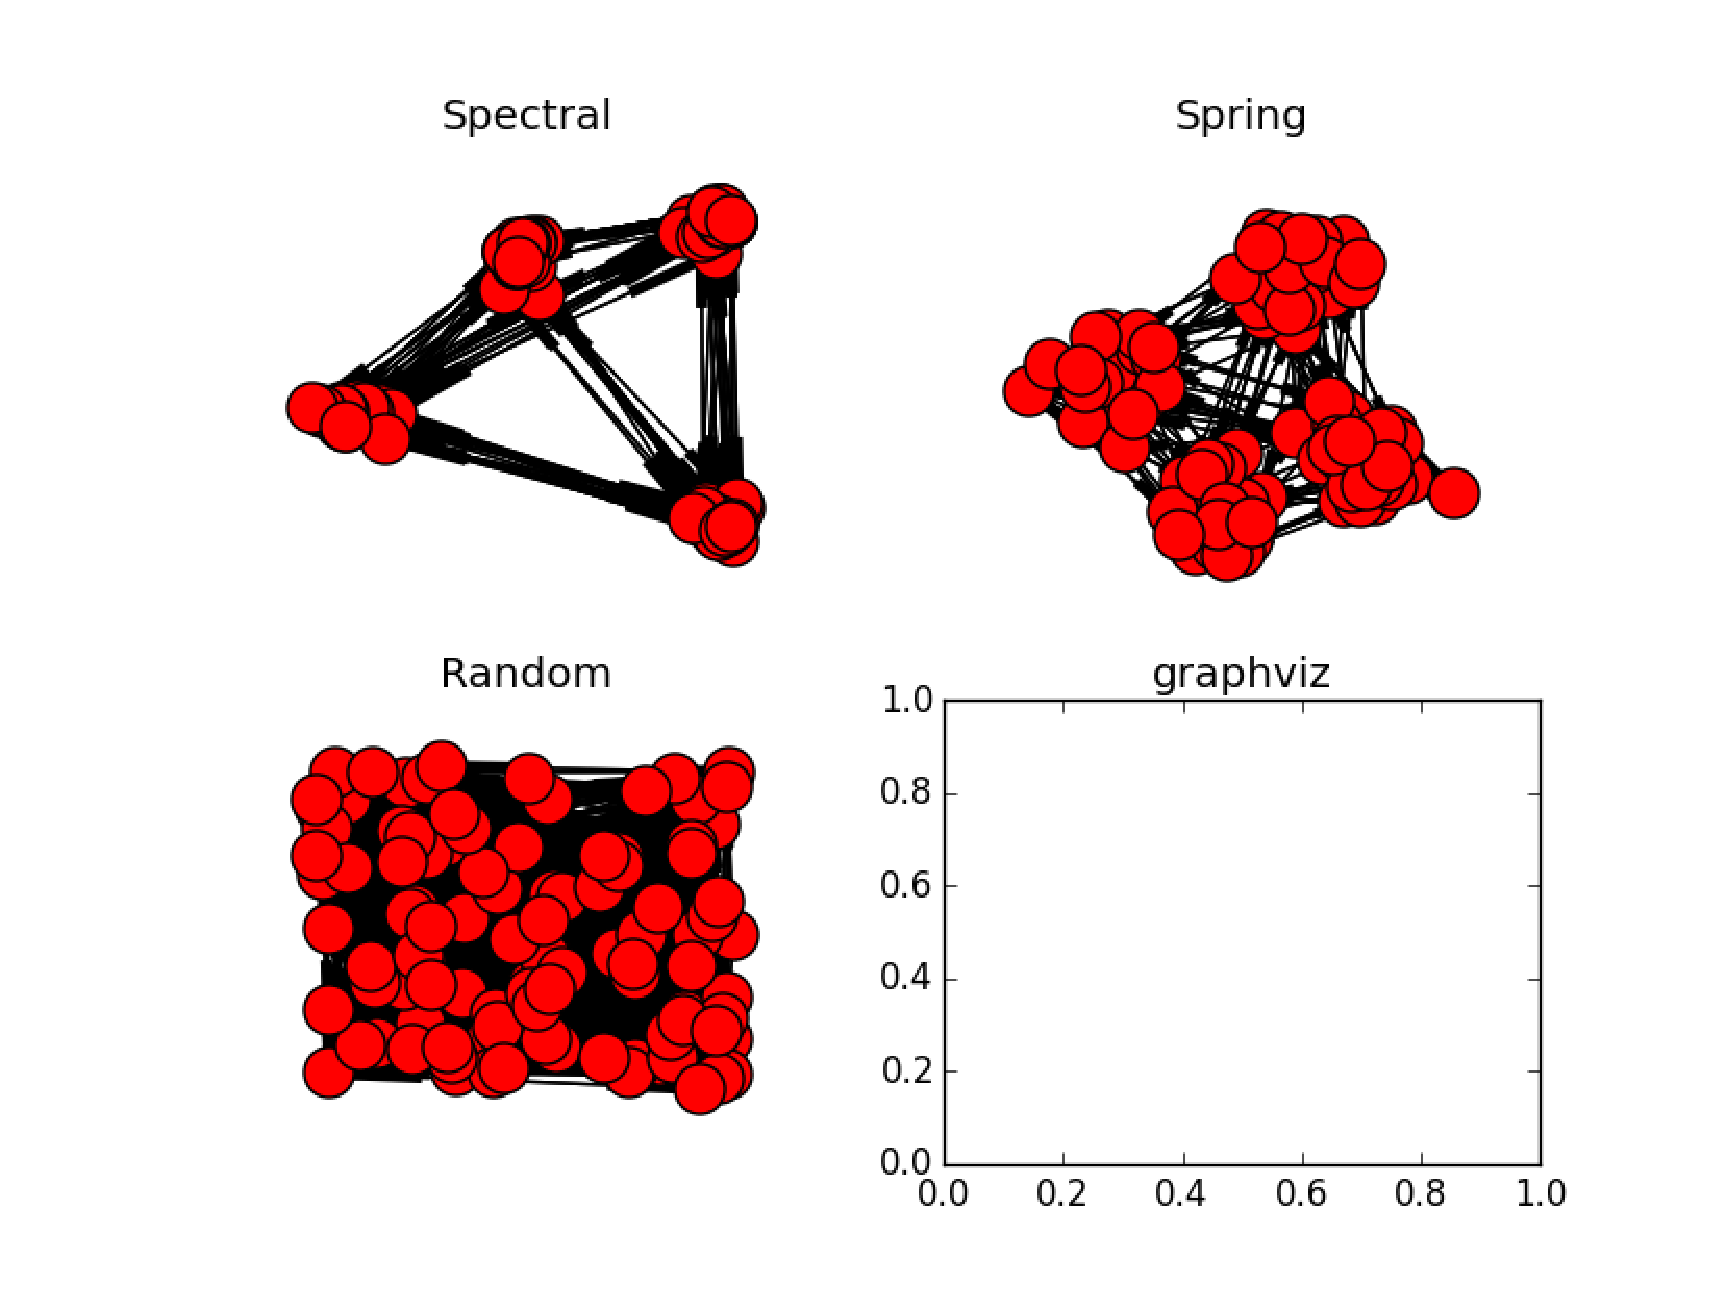
\includegraphics[scale=0.3]{img/networks}
    \end{figure}
\end{frame}

\begin{frame}[c]{Social Networks Properties}
    \textit{\Large{Important properties observed in social networks}}
    \vspace{2em}

\scalebox{0.82}{
    {\renewcommand{\arraystretch}{1.8}
    \begin{tabular}{|c|c|}
    \hline
    \textbf{Property} & \textbf{Measure} \\
    \hline
    \hline
    Small World & Diameter  (Millgram 1978, Leskovec 2008 )\\
    \hline
    Community & Modularity, Clustering Coefficient (Newman 2006) \\
    \hline
    Homophily & Homophily Coefficient (McPherson 2001) \\
    \hline
    Preferential Attachment / Burstiness & Degree Distribution (Barab\'asi 1999) \\
    \hline
    Sparsity & Density (Haldous, Hoover 1981) \\
    \hline
    \end{tabular}}
    }
\end{frame}


%
%
% Why probabilistic models.
% (who use it, why)
%
%

\begin{frame}[t]{Statement}
    \vspace{3em}

    \textit{\Large{We focus on two models in the class of Mixed-Membership Models: }}
    \begin{itemize}
        \item IMMSB (infinite Mixed-Membership Stochastic Blockmodel)
        \item ILFM (infinite Latent Feature Model) 
    \end{itemize}

    \vspace{2em}

    \textit{\Large{Do those models comply with preferential attachment? homophily?  }}


\pause

\begin{block}{Claims}
\begin{tabular}{l|cc|c}

    \multicolumn{3}{c}{\hspace{1.3cm}Preferential Attachment}   \\
    \cmidrule(l){2-3} 
    &   global & local  &   homophily      \\
    \hline
    ILFM       & \cellcolor{red!25}No & \cellcolor{red!25}No   & depends on similarity  \\
    IMMSB       & \cellcolor{red!25}No & \cellcolor{green!25}Yes  & depends on similarity \\
\end{tabular}
\end{block}

\end{frame}

\section{Probabilistic Graph Models}

%
% People like it 
%

\begin{frame}[t]{Probabilistic Model}

    % digression for recall on probabilistic modeling and bayesian reasoning

    \begin{columns}[t]
    \begin{column}{0.8\textwidth}
    \begin{block}{The Joint Distribution}
        $P(Y,\Theta \mid\sigma)$: How observations of a natural phenomena arise
    \end{block}

    \begin{block}{Likelihood}
        $P(Y \mid \Theta)$: How observations depend on the latent variables
    \end{block}

    \begin{block}{Prior}
        $P(\Theta \mid\sigma)$: Describe the latent variables of the model
    \end{block}

    \end{column}
    \begin{column}{0.25\textwidth}

        \begin{block}{Graphical Model}
            \centering
            \begin{tikzpicture}
                \node[const] (a) {$\sigma$};
                \node[latent, below=of a] (p) {$\Theta$};
                \node[obs, below=of p] (y) {$Y$};

                \edge {a}{p};
                \edge {p}{y};
            \end{tikzpicture}

        \end{block}
    \end{column}
    \end{columns}

    \pause

    \begin{columns}[t]
        \begin{column}{0.35\textwidth}
        \begin{block}{The generative process}
            \begin{align*}
                \Theta &\sim P(\Theta \mid \sigma) \\
                y &\sim P(y \mid\Theta)
            \end{align*}
        \end{block}
        \end{column}
        \begin{column}{0.65\textwidth}
        \begin{block}{Inference / Optimisation}
            Posterior Distribution: $\textcolor{blue}{P(\Theta \mid Y)}  = \frac{P(Y|\Theta)P(\Theta)}{P(Y)}$
        \end{block}
        \end{column}
    \end{columns}

\end{frame}


%\begin{frame}[c]{Predictions}
%    Predictions involve the posterior distribution (+ sum and product rules):
%
%    \begin{align}
%        p(y^{new}| Y, \sigma) &= \int_\Theta P(y^{new}|\Theta) \textcolor{blue}{P(\Theta | Y, \sigma)}\ d\Theta \\
%                              &= \mathbb{E}_{\Theta \sim P(\Theta | Y, \sigma)} [P(y^{new}|\Theta)]
%    \end{align}
%
%    \underline{\alert{NOTE}}: Assumption of conditional independancy of observations in the likelihood. (Static Networks)
%    
%\end{frame}

%\begin{frame}[t]{Regression Example (Ridge)}
%
%    Given $Y$ and $X$:
%
%    \begin{equation*}
%        Y_i = \sum_k x_k \beta_k + \varepsilon_i  \qquad (\textrm{matrix form}: Y = \bm{\beta}^T X + \mathcal{E} )
%    \end{equation*}
%
%    Find $\bm{\beta}$ ?
%
%    \pause
%
%    \begin{columns}[t]
%        \begin{column}{0.4\textwidth}
%            \vspace{-2cm}
%            \begin{align*}
%                \beta_k &\sim \mathcal{N}(0, \sigma) \\%= \frac{1}{\sqrt{2\pi\sigma }}e^{-\frac{\beta_k^2}{2\sigma}} \\
%                y_i &\sim \mathcal{N}(\beta^T X_i, \sigma_n) 
%            \end{align*}
%            \vfill
%        \end{column}
%        \begin{column}{0.5\textwidth}
%            \begin{tikzpicture}
%                \node[obs, below=of p] (y) {$Y_i$};
%                \node[obs, left=of y] (x) {$X_i$};
%                \node[latent, right=of y] (p) {$\beta_k$};
%                \node[const, above=of p] (a) {$\sigma$};
%                \node[const, above=of y] (n) {$\sigma_n$};
%
%                \edge {a}{p};
%                \edge {p}{y};
%                \edge {x}{y};
%                \edge {n}{y};
%
%                \plate {} {(x)(y)} {$N$} ;
%                \plate {} {(p)} {$K$} ;
%            \end{tikzpicture}
%
%        \end{column}
%    \end{columns}
%
%    \pause
%
%    Optimisation Problem: 
%    \begin{align*}
%        \mathrm{arg}\max\limits_{\bm{\beta}}  P(\bm{\beta}| Y, X) &= P(Y | \bm{\beta}, X) P(\bm{\beta}) \\
%        &=  \prod_i P(Y_i | \beta,  X_i) \prod_k P(\beta_k) \\
%        \mathrm{arg}\min\limits_{\bm{\beta}}  -\log(P(\bm{\beta}| Y, X))  &=  \sum_i (Y_i - \bm{\beta}^T X_i)^2  + \frac{\sigma_n}{\sigma}\sum_k \beta_k^2
%    \end{align*}
%
%\end{frame}


\begin{frame}[t]{Social Network to Graph}

    %Graph and adjacency matrix define the topology of a network.

    \begin{description}[align]
        \item[A graph]: $G = (V,E)$
            \begin{itemize}
                \item $V$: set of vertices, drawn as nodes,
                \item $E$: set of edges, drawn as lines connecting vertices,
            \end{itemize}

        \item[containing $N$ nodes]:  $|V| = N$
        \item[Define a adjacency matrix]:  $Y=(y_{ij}) \quad i,j \in V^2, \left| \substack{\ y_{ij}=1 \quad \textrm{if} \quad (i,j) \in E \\ y_{ij}=0 \quad \textrm{otherwise} } \right.\kern-\nulldelimiterspace  $
    \end{description}

    \begin{columns}
        \begin{column}{0.5\textwidth}
        \begin{figure}[h]
        \includegraphics[scale=0.25]{img/net.pdf}
        \end{figure}
        \end{column}
        \begin{column}{0.5\textwidth}
        \begin{figure}[h]
        \includegraphics[scale=0.15]{img/gdot.png}
        \end{figure}
        \end{column}
    \end{columns}
\end{frame}

%
%
% Insist on reading the matrix to the graph (it helps)
%
%


\begin{frame}[t]{Unsupervised Learning}

    % Latent variable and factorization matrix view.
    \textit{\Large{Learn a  \emph{"good"} representation of the data in order to do: }}
    \begin{itemize}
        \item Links Prediction
        \item Clustering and Visualization
    \end{itemize}


    \pause ~\\

    \begin{description}[align]
        \item[Approximate the adjacency matrix]:  $Y \approx F\Phi F^T$
    \end{description}

    \begin{columns}
        \begin{column}{0.5\textwidth}
            
\begin{tikzpicture}[scale=.5]



\node (y) [rectangle, fill=black!10, minimum height=2cm, minimum width=2cm] {$Y$};
    \node (eq) [right=0.1cm of y] {$\sim h($};
\node (p) [rectangle, fill=blue!40, minimum height=2cm, minimum width=1cm, right=0.1cm of eq] {$F$};
\node (f) [rectangle, fill=green!40, minimum height=1cm, minimum width=1cm, yshift=0.5cm , right=0.3cm of p] {$\Phi$};
\node (pt) [rectangle, fill=blue!40, minimum height=1cm, minimum width=2cm,  right=0.3cm of f] {$F^T$};
    \node (close) [yshift=-0.5cm, right=0cm of pt] {)};

\node[below of=y, yshift=-0.25cm] (Y) {$N \times N$};
\node (F) [below of=p, yshift=-0.25cm] {$N \times K$};
\node (P) [below of=f, yshift=0.1cm] {$K \times K$};


\end{tikzpicture}


        \end{column}
        \begin{column}{0.5\textwidth}
        \begin{figure}[h]
        \includegraphics[scale=0.15]{img/gdot.png}
        \end{figure}
        \end{column}
    \end{columns}

    

    \begin{description}[align]
        \item[A latent feature matrix]: $F \in \mathcal{F}^{N\times K}$ -- Local variable for each node
        \item[A latent weights matrix]:  $\Phi \in \mathcal{P}^{K\times K}$ -- Global variable shared by all nodes
    \end{description}
    \emph{Assume $K$ the dimension of the model (dimension of latent variables)}

    \begin{columns}
        \begin{column}{0.5\textwidth}
            
\begin{tikzpicture}[scale=.5]



\node (y) [rectangle, fill=black!10, minimum height=2cm, minimum width=2cm] {$Y$};
    \node (eq) [right=0.1cm of y] {$\sim h($};
\node (p) [rectangle, fill=blue!40, minimum height=2cm, minimum width=1cm, right=0.1cm of eq] {$F$};
\node (f) [rectangle, fill=green!40, minimum height=1cm, minimum width=1cm, yshift=0.5cm , right=0.3cm of p] {$\Phi$};
\node (pt) [rectangle, fill=blue!40, minimum height=1cm, minimum width=2cm,  right=0.3cm of f] {$F^T$};
    \node (close) [yshift=-0.5cm, right=0cm of pt] {)};

\node[below of=y, yshift=-0.25cm] (Y) {$N \times N$};
\node (F) [below of=p, yshift=-0.25cm] {$N \times K$};
\node (P) [below of=f, yshift=0.1cm] {$K \times K$};


\end{tikzpicture}


        \end{column}
        \begin{column}{0.5\textwidth}
        \begin{figure}[h]
        \includegraphics[scale=0.15]{img/gdot.png}
        \end{figure}
        \end{column}
    \end{columns}
\end{frame}



\begin{frame}[t]{Random Graph model}

Given a Graph $G=(V,E)$, find $\textcolor{blue}{F}$ and $\textcolor{green}{\Phi}$ such that:

\begin{equation*}
    Y \sim P(Y | \textcolor{blue}{F}, \textcolor{green}{\Phi}) = \textcolor{blue}{F}\textcolor{green}{\Phi} \textcolor{blue}{F}^T
\end{equation*}


\begin{description}
\setlength{\itemindent}{-2cm}
\item[\textcolor{blue}{$F$}]: a latent feature matrix (describe the membership of nodes)
\item[\textcolor{green}{$\Phi$}]: a latent weight matrix (describe the correlation between class)
\end{description}

\pause


    \begin{columns}
        \begin{column}{0.5\textwidth}
            \begin{block}{Likelihood}
            \[ P(y_{ij}=1 | F, \Phi) = f_i \Phi f_j^T \]
            \end{block}
            What prior over $F$ and $\Phi$ ?
        \end{column}
        \begin{column}{0.5\textwidth}
        \begin{figure}[h]
        \includegraphics[scale=0.15]{img/gdot.png}
        \end{figure}
        \end{column}
    \end{columns}

\end{frame}

\newcounter{row}
\newcounter{col}
\newcommand\setrow{}

\begin{frame}[t]{Random Graph Model (cont.)}
    The Stochastic Blockmodel \footfullcite{goldenberg2010survey}

    \begin{itemize}
        \item We have $K$ blocks and,
        \item Any node $i$ belongs to one block $c$:
        \item Each weights $\phi_{kl}$ , $k,l \in (0, .., K-1)^2$  encode the strength between two blocks.
    \end{itemize}

    ~\\
    \emph{Arbitrary Example:}

    \begin{block}{Block membership for node 4 and 7 (K=3 and N=9)}

    \begin{columns}[t]
        \begin{column}{0.45\textwidth}
        $f_4$ = \raisebox{-2pt}{%\newcounter{row}
%\newcounter{col}
\setcounter{row}{0}
\setcounter{col}{0}

\renewcommand\setrow[3]{
    \setcounter{col}{1}
    \foreach \n in {#1, #2, #3} {
        \edef\x{\value{col} -0.5}
        \edef\y{\value{row} -0.5}
        \node[anchor=center] at (\x, \y) {\n};
        \stepcounter{col}
    }
    \stepcounter{row}
}

\begin{tikzpicture}[scale=.5]

    \begin{scope}
        \draw (0, 0) grid (3, 1);
        %\draw[very thick, scale=3] (0, 0) grid (3, 3);

    \setcounter{row}{1}
        \setrow {0}{1}{0}  {0}{0}

        %\node[anchor=center] at (4.5, -0.5) {};
    \end{scope}
\end{tikzpicture}
}
        \end{column}
        \begin{column}{0.45\textwidth}
            \hspace{-1.5cm}
        $f_7$ = \raisebox{-2pt}{\input{img/feature2}}
            \hspace{0.5cm}
        $\phi_{12} = 0.3$
        \end{column}
    \end{columns}

    \end{block}

    \begin{figure}[h]
    \includegraphics[scale=0.3]{img/sb}
        \caption{Stochastic Blockmodel}
    \end{figure}
    
\end{frame}

\begin{frame}[c]{Mixed Membership Models}

    Relax the single membership assumption (soft clustering).

    \begin{block}{Binary features}
        $f_i$ = \raisebox{-2pt}{\input{img/feature3}}
    \end{block}
    Also relax the fixed number of features $K$ with an Indian Buffet Process (IBP). \\
    %And Gaussian weights...

    \vspace{0.2cm}
    \emph{or}
    \vspace{0.2cm}

    \begin{block}{Proportion features}
        $f_i$ = \raisebox{-2pt}{%\newcounter{row}
%\newcounter{col}
\setcounter{row}{0}
\setcounter{col}{0}

\renewcommand\setrow[5]{
    \setcounter{col}{1}
    \foreach \n in {#1, #2, #3, #4, #5} {
        \edef\x{\value{col}*1.2 -0.5*1.2}
        \edef\y{\value{row} -0.5}
        \node[anchor=center] at (\x, \y) {\n};
        \stepcounter{col}
    }
    \stepcounter{row}
}

\begin{tikzpicture}[scale=.5]

    \begin{scope}
        \draw[xscale=1.2] (0, 0) grid (5, 1);
        %\draw[very thick, scale=3] (0, 0) grid (3, 3);

    \setcounter{row}{1}
        \setrow {.5}{.2}{.1}{.1}{.1}

        %\node[anchor=center] at (4.5, -0.5) {};
    \end{scope}
\end{tikzpicture}
} \hspace{2em} $\sum f_i=1$
    \end{block}
    Also relax the fixed number of features $K$ with a (Hierarchical) Dirichlet Process (DP). \\
    %And beta weights...
    
\end{frame}

\begin{frame}[c]{Random Graph Model (cont.)}

    Infinite Mixed Membership Stochastic Model (IMMSB) \footfullcite{IMMSB}
    \vspace{1cm}

    \begin{columns}[t]
        \begin{column}{0.5\textwidth}
            \vspace{-5cm}
            \begin{align*}
                &\bm{\beta} \sim \textrm{GEM}(\gamma)\\
                &\textrm{For each } i \in \{1, .., N\}  \\
                &\qquad\bm{f}_i \sim \textrm{DP}(\alpha_0, \bm{\beta})\\
                &\textrm{For each }  (m,n) \in \{1,..,K\}^2 \\
                &\qquad\phi_{mn} \sim \mathrm{Beta}(\lambda_0,\lambda_1)\\
                &\textrm{For each } (i,j) \in V^2 \\
                &\qquad z_{i \rightarrow j} \sim \mbox{Mult}(\bm{f}_i)\\
                &\qquad z_{i \leftarrow j} \sim \mbox{Mult}(\bm{f}_j)\\
                &\qquad y_{ij} \sim \mathrm{Bern}({z_{i \rightarrow j} \Phi z_{i \leftarrow j}^T})
            \end{align*}
        \end{column}
        \begin{column}{0.5\textwidth}
            \scalebox{0.88}{/home/dulac/Documents/workInProgress/networkofgraphs/papers/personal/figures/draw/mmsb2.tex}
        \end{column}
    \end{columns}

\end{frame}

\begin{frame}

    Infinite Latent Feature Model (ILFM) \footfullcite{ILFRM}
    \vspace{1cm}

    \begin{columns}[t]
        \begin{column}{0.5\textwidth}
            \vspace{-4cm}
            \begin{align*}
                &F \sim \textrm{IBP}(\alpha)\\
                &\textrm{For each }  (m,n) \in \{1,..,K\}^2 \\
                &\qquad\phi_{mn} \sim \mathrm{Gaussian}(0,\sigma_w)\\
                &\textrm{For each } (i,j) \in V^2 \\
                &\qquad y_{ij} \sim \mathrm{Bern}(\bm{f}_i \Phi \bm{f}_j^T)
            \end{align*}
        \end{column}
        \begin{column}{0.5\textwidth}
            \scalebox{0.88}{/home/dulac/Documents/workInProgress/networkofgraphs/papers/personal/figures/draw/ilfrm2.tex}
        \end{column}
    \end{columns}
\end{frame}

\section{Properties Characterization}

\begin{frame}[c]{Preferential Attachment}

    \[ \Delta_n P(d_i \geq n+1 | d_i \geq n) > 0 \]

    \begin{figure}[h]
        \caption{power law distribution in empirical data}
    \includegraphics[scale=0.25]{img/power_law.pdf}
    \end{figure}

    \footfullcite{clauset2009power}
\end{frame}

\begin{frame}[c]{Characterisation of Burstiness}

    Three Levels.


    \begin{columns}[t]
        \begin{column}{0.5\textwidth}
            \begin{definition}{Global Preferential attachment}
                \[ \Delta_n P(d_i \geq n+1 | d_i \geq n) > 0 \]
            \end{definition}
            \begin{definition}{Local Preferential attachment}
                \[ \Delta_n P(d_{ic} \geq n+1 | d_{ic} \geq n) > 0 \]
            \end{definition}
            \begin{definition}{Feature Burstiness}
                \[ \Delta_n P(\bm{f}_k \geq n+1 | \bm{f}_k \geq n) > 0 \]
            \end{definition}
        \end{column}
        \begin{column}{0.5\textwidth}

        \begin{figure}[h]
        \includegraphics[scale=0.25]{img/gdot.png}
        \end{figure}

        \end{column}
    \end{columns}

\end{frame}



\section{Results and Illustrations}

\begin{frame}[c]{Theoretical Results}

    Summary of our theoretical results. \footfullcite{A study of stochastic mixed membership models for link prediction in social networks: Under Revision}
    \vspace{1cm}


    \begin{block}{Theoretical results}
	\begin{tabular}{l|cc|c}

        \multicolumn{3}{c}{\hspace{1.3cm}Preferential Attachment}   \\
        \cmidrule(l){2-3} 
        &   global & local  &   homophily      \\
        \hline
        ILFM       & \cellcolor{red!25}No & \cellcolor{red!25}No   & depends on similarity  \\
        IMMSB       & \cellcolor{red!25}No & \cellcolor{green!25}Yes  & depends on similarity \\
    \end{tabular}

    \end{block}

\end{frame}

\begin{frame}[c]{Empirical Results (I)}

    \vspace{-0.2cm}

    \begin{columns}[t]
        \begin{column}{0.5\textwidth}
        \begin{figure}[h]
            \caption{Synthetic Datasets.}
        \includegraphics[scale=0.2]{img/burst_sint.pdf}
        \end{figure}
        \end{column}
        \begin{column}{0.5\textwidth}
        \begin{figure}[h]
            \caption{Prediction Performance, AUC curves.}
        \includegraphics[scale=0.25]{img/auc.pdf}
        \end{figure}
        \end{column}
    \end{columns}

\end{frame}

\begin{frame}[c]{Empirical Results (II)}
        \begin{figure}[h]
            \caption{Comparison performance of IMMSB and ILFM based on the size of the training set.}
        \includegraphics[scale=0.5]{img/testset_max_20_roc_evolution}
        \end{figure}
\end{frame}


\section{Limitation and Future Work}

\begin{frame}[c]{Limitation and future work}
    Representation Theorem for exchangeable graph \footfullcite{orbanz2015bayesian}.

    \begin{block}{Aldous-Hoover Theorem}
        An array $(Y_{ij})_{{ij}\in \mathbb{N}}$ is jointly exchangeable if and only if :
    \begin{equation}
        Y_{ij} \sim F(U_i, U_j, U_{ij})
    \end{equation}

    \begin{itemize}
        \item With $F: [0,1]^3 \rightarrow [0,1]$ a random measure, 
        \item  $(U_i)_{i\in \mathbb{N}}$ and $(U_{{ij}\in \mathbb{N}})$   i.i.d Uniform[0,1] random variables.
    \end{itemize}
    \end{block}

    A corollary of this theorem is that random exchangeable graph are either \textbf{empty or dense}.
    \vspace{1cm}

    \MVRightarrow{} What network structure and invariance to comply with the Global preferential attachment ?

\end{frame}


\begin{frame}[c]{Conclusion}
    \begin{block}{Wrap up}
    \begin{itemize}
        \item Formal Definition of social networks properties [Homophily and Preferential Attachments].
        \item Study of compliance of Mixed Membership Models with the properties.
        \item Empirical implications on prediction performances.
    \end{itemize}
    \end{block}

    \begin{block}{Future work}
    \begin{itemize}
        \item Extend to weighted networks (and scalable inference).
        \item Extend to temporal networks. 
    \end{itemize}
    \end{block}
\end{frame}

\begin{frame}[c]{Bottom}
    \textcolor{green}{Thank You}
\end{frame}

%
%
%
%
%
%
%
%

\begin{frame}[c]{Characterisation of Burstiness (cont .)}

    Generative Process for IMMSB.

        \begin{figure}[h]
            \caption{IMMSB Simulation.}
        \includegraphics[scale=0.2]{img/mmsb_burst.pdf}
        \end{figure}
\end{frame}

%\begin{frame}[c]{Characterisation of Burstiness (cont .)}
%
%    Generative Process for ILFM.
%
%        \begin{figure}[h]
%        \includegraphics[scale=0.2]{img/ilfm_burst.pdf}
%            \caption{ILFM Simulation.}
%        \end{figure}
%\end{frame}

\begin{frame}[c]{Characterisation of Burstiness (cont .)}

    Is there a proof ?

    \[ P(d_i=n | \alpha) \quad ?\]
    \begin{block}{Problem}
        \begin{itemize}
            \item $d_i$ random variable ?
            \item $P(\bm{Y}_i \mid \alpha, \lambda) = \int_F \int_\Phi p(f_i| \alpha)p(\Phi|\lambda) \prod_{j\neq i} p(f_j|\alpha) p(y_{ij} \mid f_i, f_j, \Phi) \ dF d\Phi$
        \end{itemize}
    \end{block}

    \alert{Intractable}...
\end{frame}


\end{document}
